\section{Wyznaczanie trajektorii dla pojedynczego robota}
\label{ch:alg-single-astar}

Wiele technik planowania tras, mimo iż może posłużyć do koordynacji ruchu wielu robotów, korzysta z metod indywidualnego planowania dla każdego agenta z osobna. Przykładem takiego podejścia jest {\it Local-Repair A*}, w którym to głównym algorytmem przeszukującym jest A*.
Z tego powodu przed przystąpieniem do opracowania bardziej skomplikowanych metod, należy najpierw zająć się implementacją algorytmu poszukiwania najkrótszej drogi na dwuwymiarowej mapie z jednym robotem. Wymagane jest to nawet dla metody WHCA*, która pomimo, że operuje na węzłąch określonych w czasie i przestrzeni, to jednak w obliczaniu samej heurystyki wykorzystuje przestrzenny algorytm A*.
Ogólna zasada działania algorytmu A* wraz z kluczowymi pojęciami została opisana w rozdziale \ref{ch:astar-theory}.

Pseudokod \ref{alg:astar} oraz opisy użytych pomocniczych funkcji ukazują szczegóły implementacji metody wyznaczania najkrótszej drogi na przestrzennej mapie. Algorytm oparty jest o A*, jednak posiada pewne własne, niewielkie modyfikacje.

\begin{algorithm}[H]
	\caption{Algorytm A*}\label{alg:astar}
  \begin{algorithmic}[1]
\Function{znajdzDrogę}{$mapa$, $start$, $cel$}
	\State $closed \gets \varnothing$  \Comment{pusta lista zamkniętych}
	\State $open \gets \{start\}$ \Comment{lista otwartych zawiera punkt startowy}

	\For{$wezel \in mapa$}
		\State $wezel.g = \infty$ \Comment{domyślnie nieskończony koszt - odległość od startu}
	\EndFor

	\State $start.g \gets 0$ \Comment{Zerowy koszt przejścia do węzła startowego}

	\While{$open \ne \varnothing$} \Comment{dopóki lista otwartych nie jest pusta}
		\State $obecny \gets $ \Call{znajdźMinF}{$open$} \Comment{Szukamy pola o najniższej wartości f}

		\If{$obecny == cel$}
			\State \Return \Call{zbudujŚcieżkę}{$cel$} \Comment{Znaleziono ścieżkę}
		\EndIf

		\State dodaj $obecny$ do $closed$ \Comment{Przesunięcie z $open$ do $closed$}
		\State usuń $obecny$ z $open$
		
		\For{$sasiad \in$ \Call{sąsiedzi}{$obecny$}} \Comment{Dla każdego sąsiada aktualnego pola}
			
			\If{$mapa[sasiad.x][sasiad.y] == ZABLOKOWANE$ {\bf or} 
				\State {\bf not} \Call{przejściePoprawne}{$obecny$, $sasiad$}}
				\State {\bf continue} \Comment{Ignoruj niepoprawne pola lub przejścia}
			\EndIf
			
			\State $nowyKoszt \gets obecny.g \ +$ \Call{kosztPrzejścia}{$obecny$, $sasiad$}

			\If{$nowyKoszt < sasiad.g$} \Comment{znaleziono korzystniejsze połączenie}
				\State usuń $sasiad$ z $open$ \Comment{konieczność ponownego przeliczenia}
				\State usuń $sasiad$ z $closed$ \Comment{jeśli $sasiad \in open$ lub $sasiad \in closed$}
			\EndIf

			\If{$sasiad \not\in open \land sasiad \not\in closed$}
				\State $sasiad.g \gets nowyKoszt$ \Comment{zapisanie nowego połączenia}
				\State $sasiad.h \gets$ \Call{heurystyka}{$sasiad$, $cel$}
				\State $sasiad.parent \gets obecny$ \Comment{pole $obecny$ rodzicem dla pola $sasiad$}
				\State dodaj $sasiad$ do $open$
			\EndIf

		\EndFor
	\EndWhile

	\State \Return $\varnothing$ \Comment{Przeanalizowano wszystkie węzły, brak istniejącej ścieżki}
\EndFunction
  \end{algorithmic}
\end{algorithm}

Wykorzystane zostały pomocnicze funkcje:
\begin{itemize}
	\item \textsc{znajdźMinF}($lista$) - Funkcja zwraca z listy pole o najniższej wartości $f$ (sumie kosztu i heurystyki);
	\item \textsc{zbudujŚcieżkę}($cel$) - Funkcja zwraca ścieżkę z punktu startowego do punktu $cel$ zbudowaną na podstawie przechodzenia wstecz od punktu $cel$ po kolejnych rodzicach węzłów, aż do dotarcia do węzła bez rodzica (punktu startowego).
	\item \textsc{sąsiedzi}($pole$) - Funkcja zwraca zbiór pól bezpośrednio sąsiadujących (dla których istnieje możliwość przejścia) ze wskazanym polem. Jest to zazwyczaj zbiór ośmiu sąsiadujących pól. Na granicach mapy należy uwzględniać warunki brzegowe.
	\item \textsc{przejściePoprawne}($poleZ$, $poleDo$) - Funkcja zwraca prawdę wtedy i tylko wtedy, gdy istnieje możliwość przejścia z $poleZ$ do $poleDo$. Gdy wykonywany jest ruch ukośny, ale na przynajmniej jednym polu sąsiadującym z $poleZ$ i $poleDo$ znajduje się przeszkoda, to taki ruch jest niepoprawny. Ruch ukośny agenta z punktu $(x_1, y_1)$ do $(x_2, y_2)$ możliwy jest tylko w przypadku, gdy na żadnym z czterech pól: $(x_1, y_1)$, $(x_2, y_1)$, $(x_1, y_2)$, $(x_2, y_2)$ nie znajduje się przeszkoda. W rzeczywistym środkowisku zabezpiecza to robota przed uderzaniem o wystający róg ściany.
	\item \textsc{kosztPrzejścia}($poleZ$, $poleDo$) - Funkcja zwraca koszt przejścia z $poleZ$ do $poleDo$. Jest to odległość w sensie metryki euklidesowej.
	\item \textsc{heurystyka}($poleZ$, $poleDo$) - Funkcja zwraca przewidywaną długość pozostałej drogi od $poleZ$ do $poleDo$. Jest to również odległość euklidesowa.
\end{itemize}

Potwierdzeniem poprawności zaimplementowania algorytmu wyznaczania najkrótszej ścieżki jest przykładowa droga przedstawiona na rysunku \ref{fig:robopath-astar-simple} pochodzącym z aplikacji. Warto zauważyć, że możliwy jest ruch ukośny robota, ale nie taki, który powodowałby kolizję z wystającym rogiem "ściany".

\begin{figure}
	\centering
	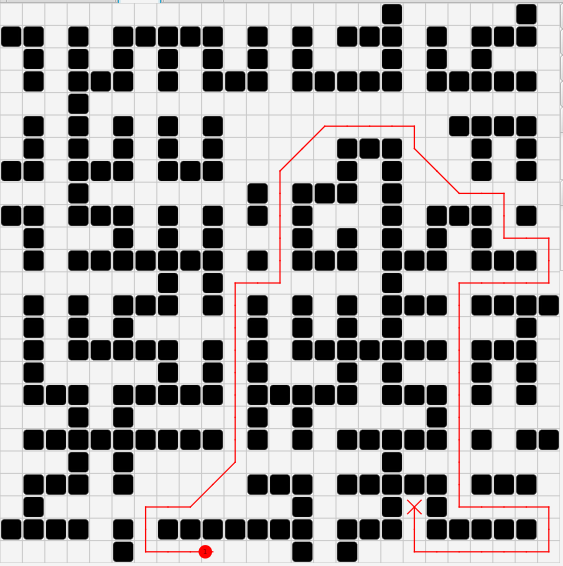
\includegraphics[width=0.5\columnwidth]{img/robopath/astar-simple}
	\caption{Przykładowa ścieżka wyznaczona przez zaimplementowany w aplikacji algorytm A*. Kolorowe koło reprezentuje robota, kolorowe koło - robota, linia łamana - wyznaczoną ścieżkę, czarne kwadraty - przeszkody.}
	\label{fig:robopath-astar-simple}
\end{figure}

% https://en.wikipedia.org/wiki/A*_search_algorithm
